\documentclass{beamer}

\usepackage{beamerthemesplit}
\usetheme{Singapore} %Copenhagen}

\input{../../include/preamble.inc} 
\input{../../include/definitions.inc} 
\input{../../include/author.inc} 

\usepackage{pgffor}

\title[]{Тензоры деформаций}

\begin{document}
	
\frame[plain]{\titlepage}


\frame[plain]{
	\frametitle{Аннотация}
	\parbox{\textwidth}{
		Движение сплошной среды. Сопутствующий базис. Метрический тензор. Нелинейный тензор деформаций. Геометрическая интерпретация компонентов тензора деформаций. Главные деформации и инварианты. Связь между относительным изменением объема и инвариантами тензора деформаций. 
	}
}




\foreach \n in {
00, 01, 02, 03, 04, 05, 06, 07, 08, 09,
10, 11, 12, 13, 14, 15, 16, 17, 18, 19,
20, 21, 22, 23, 24, 25, 26, 27, 28, 29,
30, 31, 32, 33, 34, 35, 36, 37, 38, 39}
{
	
\frame{
	\frametitle{ Пример деформации сплошной среды }
	
	\centering
	\includegraphics[width=11cm]{../img/example/fig_\n.pdf}
	
	\bigskip
	Лагранжево и эйлерово представление

}

}


\frame{
	\frametitle{ Траектории движения точек }
	
	\centering
	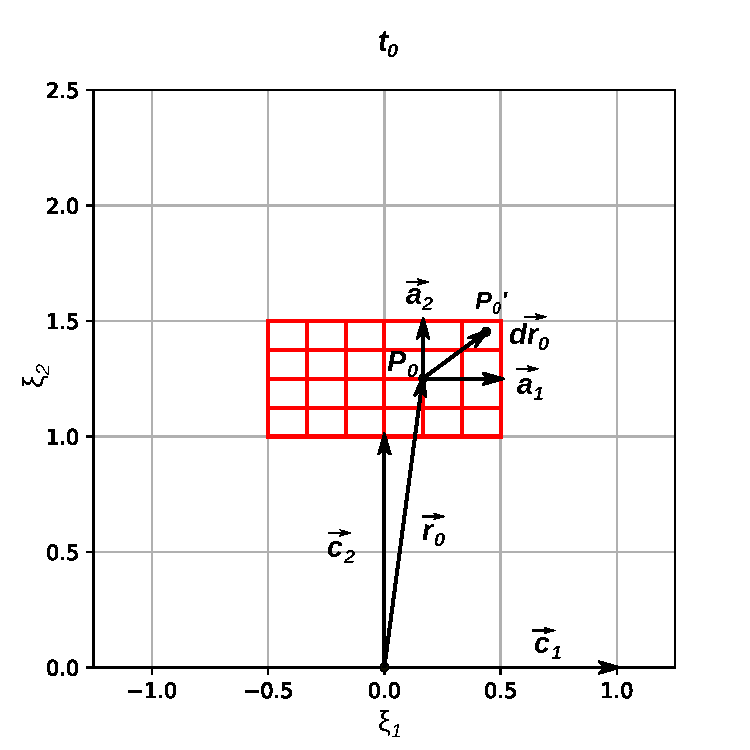
\includegraphics[width=5cm]{../img/state_0_00.pdf}~
	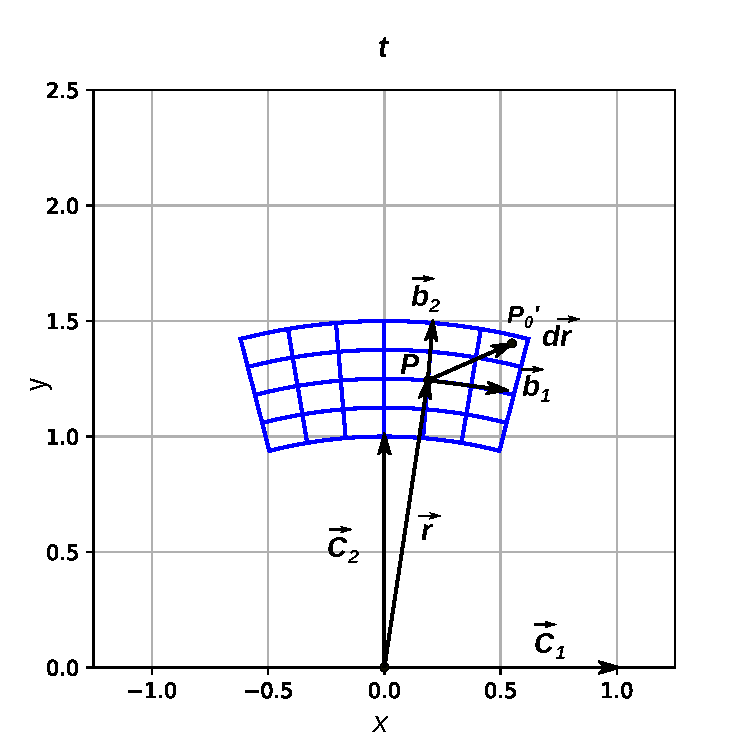
\includegraphics[width=5cm]{../img/state_0_50.pdf}
	
	\begin{exampleblock}{}
		\parbox{\textwidth}{
			Пусть задан закон деформирования тела в неподвижной фиксированной системе отсчета
			$x^i = x^i\argtxi$, 	обладающий свойст\-вом гладкости и обратимости.
		}
	\end{exampleblock}
	
}

\frame{
	\frametitle{ Базис неподвижной системы координат }
	\centering

	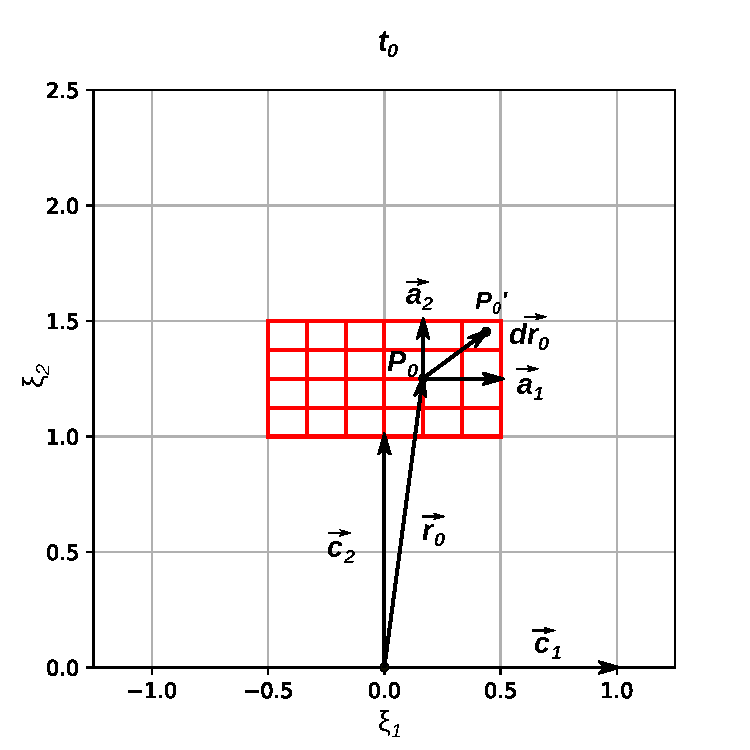
\includegraphics[width=4cm]{../img/state_0_00.pdf}~
	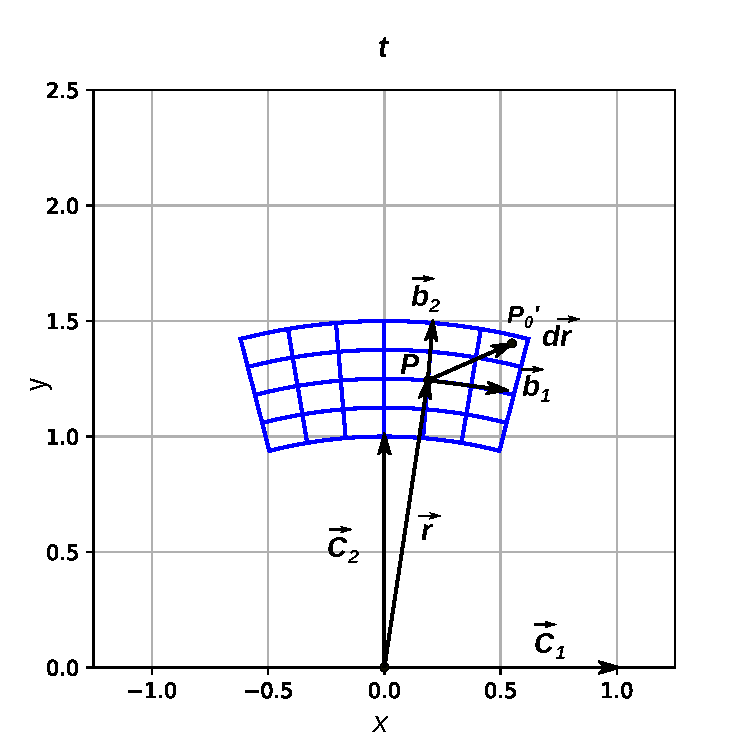
\includegraphics[width=4cm]{../img/state_0_50.pdf}	
	
	\begin{exampleblock}{Определение}
		\parbox{\textwidth}{
			Координаты произвольной точки $P$ в абсолютной декартовой сис\-теме координат представляются в виде
			\[
				\vec{r}= \vec{c}_i x^i\argtxi,
			\]
			где $\vec{c}_i$ -- базис абсолютной системы координат.
		}
	\end{exampleblock}
}

\frame{
	\frametitle{ Сопровождающий базис }
	\centering

	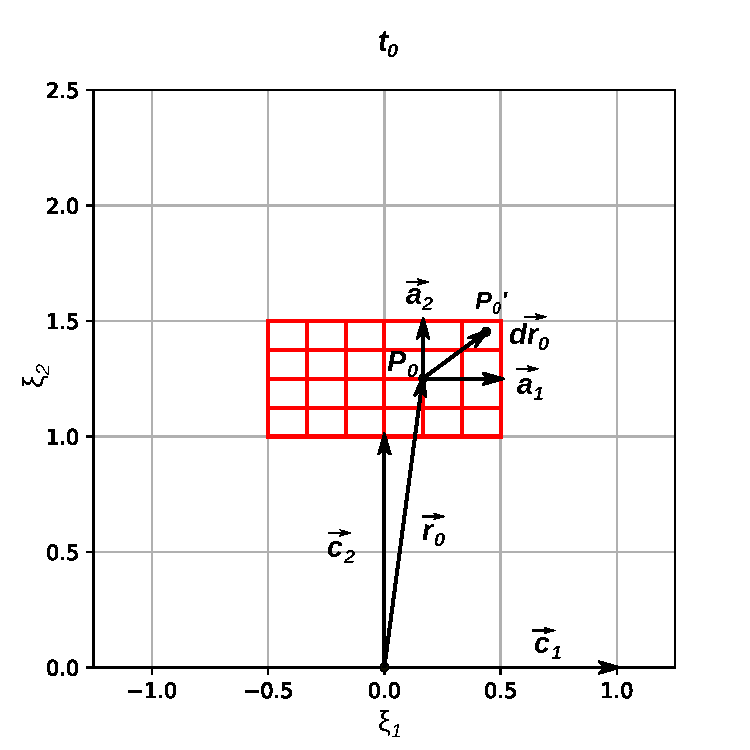
\includegraphics[width=4cm]{../img/state_0_00.pdf}~
	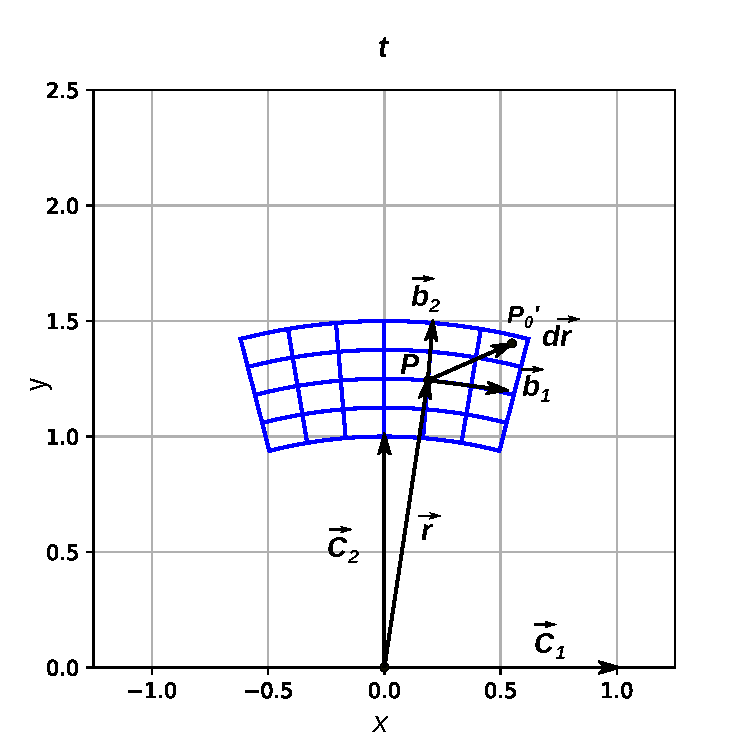
\includegraphics[width=4cm]{../img/state_0_50.pdf}	
		
	\small
	\begin{exampleblock}{Определение}
		\parbox{\textwidth}{
			Базисные векторы $\vec{b}_j$ в движущейся системе координат задаются формулами:
			\[
			\vec{b}_j = \pd{\vec{r}}{\xi^j}=\vec{c_i}\pd{x^i\argtxi}{\xi^j},
			\]
			причем эти векторы зависят не только от координат точки $\argxi$, но и от времени $t$.
		}
	\end{exampleblock}
	
}

\frame{
	\frametitle{ Сопровождающий базис при $t=t_0$ }

	\centering

	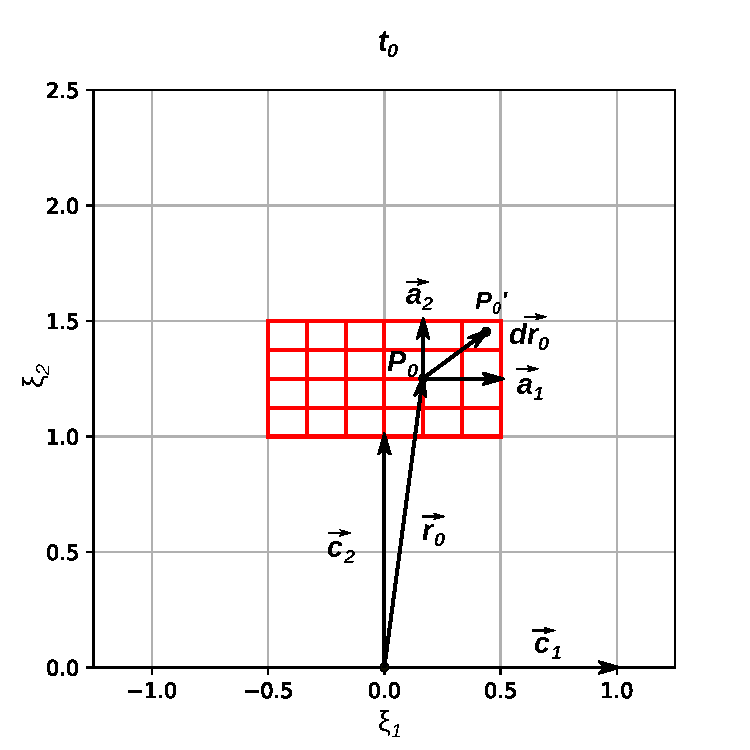
\includegraphics[width=4cm]{../img/state_0_00.pdf}~
	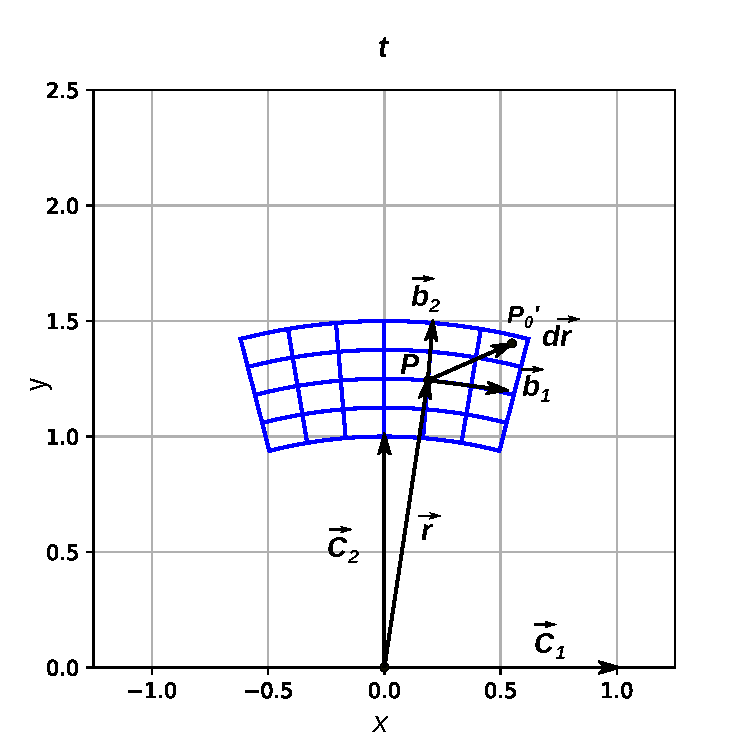
\includegraphics[width=4cm]{../img/state_0_50.pdf}	
	
%	\small
	\begin{exampleblock}{Определение}
		\parbox{\textwidth}{
			Базисные векторы в движущейся системе координат при $t=t_0$ будем обозначать $\vec{a}_j$:
			\[
			\vec{a}_j = \pd{\vec{r}_0}{\xi^j} = \vec{c_i} \pd{x^i \argtoxi }{\xi^j}.
			\]
		}
	\end{exampleblock}
}

\frame{
	\frametitle{ Метрический, или фундаментальный, тензор при $t=t_0$}
	
	\parbox{\textwidth}{
		Пусть точка $P_0'$ находится в окрестности точки $P_0\argxi$. Вектор $P_0P_0' = d\vec{r}_0$ может быть представлен в виде
		\[
		d\vec{r}_0=\vec{a}_i d\xi^i,
		\] 
		а квадрат элемента дуги $ds_0$ как
		\[
		(ds_0)^2=d\vec{r}_0 \cdot d\vec{r}_0 = \vec{a}_i\cdot\vec{a}_j d\xi^i d\xi^j,
		\]
		или 
		\[
		(ds_0)^2 = h_{ij} d\xi^i d\xi^j,
		\]
		где $h_{ij}=\vec{a}_i\cdot\vec{a}_j$ -- \alert{метрические коэффициенты} при $t=t_0$.
	}

}

\frame{
	\frametitle{ Метрический, или фундаментальный, тензор в общем случае }
	\parbox{\textwidth}{
		Пусть при деформации точка $P_0$ перешла в точку $P$, а $P_0'$ в точку $P'$, тогда вектор $P_0P_0' = d\vec{r}_0$ перейдет в вектор  $PP' = d\vec{r}$.
		
		\medskip
		Квадрат элемента дуги $ds$, определяемый вектором $PP'=d\vec{r}=\vec{b}_id\xi^i$, имеет вид
		\[
		ds^2=\vec{b}_i \cdot \vec{b}_j d\xi^i d\xi^j,
		\]
		или 
		\[
		ds^2 = g_{ij} d\xi^i d\xi^j,
		\]
		где  $g_{ij}=\vec{b}_i\cdot\vec{b}_j$ -- \alert{метрические коэффициенты} при произвольном $t$.
	}
}

\frame{
	\frametitle{ Тензор деформаций }
	
	\begin{exampleblock}{Определение}
		\parbox{\textwidth}{
			Будем говорить, что среда находится в \alert{состоянии деформации-напряжения}, если $ds_0 \neq ds$.	 \pause		
			В качестве меры деформирования можно принять 
			\[
			(ds)^2-(ds_0)^2 = (g_{ij}-h_{ij}) d\xi^i d\xi^j = 2\varepsilon_{ij} d\xi^i d\xi^j,
			\]
			где  $g_{ij}-h_{ij} = 2\varepsilon_{ij}$.
			По ранее доказанным теоремам $\varepsilon_{ij}$ -- тензорная величина и называется \alert{нелинейным тензором деформаций}.
		}
	\end{exampleblock}\pause
	
	\begin{exampleblock}{Симметричность}
		\parbox{\textwidth}{
			\[
			\varepsilon_{ij} = \varepsilon_{ji}
			\]
		}
	\end{exampleblock}
	
}
\frame{
	\frametitle{ Различные представления тензора деформаций }
	
	
	\begin{exampleblock}{Определение}
		\parbox{\textwidth}{
			Полученную тензорную величину можно расписать покомпонентно как в базисе состояния $t_0$:
			\[
			E_0 = \varepsilon_{ij}\vec{a}^i\vec{a}^j,
			\]
			так и в базисе состояния $t$:
			\[
			E = \varepsilon_{ij}\vec{b}^i\vec{b}^j.
			\]
			В первом случае имеет место представление Альманси, во втором~--- Грина. 
		}
	\end{exampleblock}
}

\frame{
	\frametitle{ Некоторые замечания }
	
	\parbox{\textwidth}{
		Опускание и поднимание индексов у тензорной величины $\varepsilon_{ij}$ происходит с помощью метрического тензора $h_{ij}$:
		\[
			h^{ij}\varepsilon_{ik} = \varepsilon^j_k, \quad
			g^{ij}\varepsilon_{ik} = \varepsilon^j_k.
		\]
		
		Однако две системы функций, вычисленных указанным путем, остаются различными, поэтому будем обозначать:
		\[
		g^{ij}\varepsilon_{ik} = \varepsilon^j_{0k}.
		\]
	}
	
	
}


\frame{
	\frametitle{ Удлинение для $E_0$}
	
	\begin{exampleblock}{Определение}
		\parbox{\textwidth}{
			Назовем \alert{удлинением $e$} изменение длины на единицу длины вектора $d\vec{r}_0=P_0P_0'$ так, что
			\[
			e=\frac{|d\vec{r}|-|d\vec{r}_0|}{|d\vec{r}_0|}=\frac{ds-ds_0}{ds_0}.
			\]
		}
	\end{exampleblock}	\pause

	Из этого выражения следует, что
	\[
	|d\vec{r}|=(1+e)|d\vec{r}_0|.
	\]\pause
	
	\begin{exampleblock}{Определение}
		\parbox{\textwidth}{
			\alert{Удлинения  $e_i$} в направлении базисных векторов $\vec{a}_i$ задаются формулой
			\[
				|\vec{b}_i|=(1+e_i)|\vec{a}_i|.
			\]
			
			
		}
	\end{exampleblock}
	
}

\frame{
	\frametitle{ Связи между удлинениями и компонентами тензора деформаций $E_0$ }
	
	\parbox{\textwidth}{
		По определению метрических тензоров $|\vec{b}_i| = \sqrt{g_{ii}}$ и $|\vec{a}_i| = \sqrt{h_{ii}}$, поэтому
		\[
			\sqrt{g_{ii}} = (1+e_i)\sqrt{h_{ii}}.
		\]\pause
		По определению тензора деформаций
		\[
		2\varepsilon_{ij} = g_{ij}-h_{ij} = \vec{b}_i\cdot\vec{b}_j - \vec{a}_i\cdot\vec{a}_j = 
		|\vec{b}_i| |\vec{b}_j| \cos\theta_{ij} - |\vec{a}_i| |\vec{a}_j| \cos{\theta_{ij}^0},
		\]
		где $\theta_{ij}$, $\theta_{ij}^0$ -- углы между базисными векторами $\vec{b}_i$, $\vec{b}_j$ и $\vec{a}_i$, $\vec{a}_j$.  \pause
		
		Следовательно,
		\[
		\frac{2\varepsilon_{ij}}{\sqrt{h_{ii}}\sqrt{h_{jj}}} = (1+e_i)(1+e_j)\cos\theta_{ij}-\cos\theta_{ij}^0.
		\]
		
	}

	
}

\frame{
	\frametitle{Связи между удлинениями и компонентами тензора деформаций  $E_0$ в случае малых удлинений }
	\parbox{\textwidth}{
		Поскольку $\theta_{ij}=\theta_{ij}^0=0$ для $i=j$, тогда
		\[
		\frac{2\varepsilon_{ii}}{h_{ii}} = (1+e_i)^2 - 1,
		\]
		или 
		\[
		e_i = \sqrt{1+\frac{2\varepsilon_{ii}}{h_{ii}}} - 1.
		\]\pause
	
		Если координаты начального состояния прямоугольные и декартовы, то $h_{ii}=1$. В случае малых деформаций, когда $2\varepsilon_{ii}/h_{ii} \ll 1$, 
		\[
			e_i \approx \varepsilon_{ii}.
		\]
		Таким образом, величины $\varepsilon_{11}$, $\varepsilon_{22}$, $\varepsilon_{33}$ связаны с удлинением дуг, направленных вдоль базисных векторов $\vec{a}_1$, $\vec{a}_2$, $\vec{a}_3$.
	}
}

\frame{
	\frametitle{ Геометрический смысл недиагональных значений тензора деформаций  $E_0$ }
	
	\parbox{\textwidth}{
		Если рассмотреть случай, когда деформация происходит из состояния, в котором система векторов $\vec{a}_i$ является ортонормированной, то будет $h_{ii}=1$, а $\theta_{ij}^0 = \pi/2$, если $i \neq j$. Пусть $\theta_{ij}=\pi/2-\alpha_{ij}$, тогда из полученных соотношений
		\[
		2\varepsilon_{ij} = (1+e_i)(1+e_j)\sin\alpha_{ij},
		\]
		или
		\[
		\sin\alpha_{ij}=\frac{2\varepsilon_{ij}}{\sqrt{1+2\varepsilon_{ii}}\sqrt{1+2\varepsilon_{jj}}}.
		\]
		

	}
	
	
}

\frame{
	\frametitle{Геометрический смысл недиагональных значений тензора деформаций  $E_0$  в случае малых деформаций }
	
	\parbox{\textwidth}{
	В случае, когда $2\varepsilon_{ii} \ll 1$ и угол $\alpha_{ij}$ мал, получается
	\[
	\alpha_{ij} \approx 2\varepsilon_{ij}.
	\]	\pause
	Таким образом, функции $\varepsilon_{ij}$ для $i \neq j$ указывают меру уменьшения первоначального прямого угла между  параллельными векторам $\vec{a}_i$ и $\vec{a}_j$ элементами дуги.\pause
	
	\bigskip
	Компоненты $\varepsilon_{ij}$ для $i\neq j$ называются \alert{скалывающими (сдвиговыми)}  компонентами тензора деформаций $E_0$. Компоненты $\varepsilon_{ii}$ -- \alert{нормальными} компонентами тензора $E_0$.
	}
	
}

\frame{
	\frametitle{ Геометрический смысл компонентов тензора $E$  }
\parbox{\textwidth}{
	По аналогии для $E=\varepsilon_{ij}\vec{b}_i\vec{b}_j$, определим удлинение $e$ как
	\[
	e=\frac{ds-ds_0}{ds},
	\]
	тогда
	\[
	e_i=1-\sqrt{1-\frac{2\varepsilon_{ii}}{g_{ii}}}
	\]
	или
	\[
	\sin\beta_{ij}=\frac{2\varepsilon_{ij}}{\sqrt{1-2\varepsilon_{ii}}\sqrt{1-2\varepsilon_{jj}}},
	\]
	где $\beta_{ij}=\theta_{ij}-\pi/2$.\pause
	 
	\medskip
	Аналогично в данном случае диагональные элементы $\varepsilon_{ii}$ ассоциируются с \alert{удлинением дуги} вдоль базисных векторов $\vec{b}_i$, а недиагональные $\varepsilon_{ij}$ соответствуют \alert{сдвиговым} деформациям.
	
}


	
	
}

\frame{
	\frametitle{ Квадратичная форма для тензора $E$ }
	
	\parbox{\textwidth}{
			Определяющая формула для компонентов тензора $\varepsilon_{ij}$ тензора деформаций $E=\varepsilon_{ij}\vec{b}_i\vec{b}_j$:
			\[
			\frac{(ds)^2-(ds_0)^2}{2(ds)^2} = \varepsilon_{ij}\frac{d\xi^i}{ds}\frac{d\xi^j}{ds},
			\]
			где $d\xi^i/ds=\lambda^i$ -- единичный вектор, определяющий направление вектора $d\vec{r}$ в конечном состоянии. \pause
			
			\medskip
			Введем в рассмотрение квадратичную форму
			\[
			Q(\lambda) = \varepsilon_{ij}\lambda^i\lambda^j
			\]
			и найдем максимальное значение этой квадратичной формы при
			\[
				\varphi(\lambda) = g_{ij}\lambda^i\lambda^j - 1 = 0.
			\]
	}
	

	
}

\frame{
	\frametitle{ Главные деформации тензора $E$ }
	
	\parbox{\textwidth}{
	
	При использовании метода множителей Лагранжа задача сводится к отысканию решения:
	\[
	\pd{Q}{\lambda^i}-\varepsilon\pd{\varphi}{\lambda^i} = 0
	\]
	или 
	\begin{equation}
	\label{eq:eps_cond}
	(\varepsilon_{ij}- \varepsilon g_{ij})\lambda^j = 0,
	\end{equation}
	где $\varepsilon$ -- множитель Лагранжа.
	
	Эта система имеет нетривиальное решение относительно $\lambda^j$, если 
	\[
	|\varepsilon_{ij} - \varepsilon g_{ij}| = 0.
	\]

	}
	
}

\frame{
	\frametitle{ Главные деформации и инварианты тензора E}
	
	\parbox{\textwidth}{
		

	
	Поднимая индекс в выражении (\ref{eq:eps_cond}) с помощью $g^{ik}$, получим:
	\[
	(\varepsilon_j^k - \varepsilon \delta_j^k)\lambda^j = 0,
	\]
	где $\varepsilon_j^k = g^{ik}\varepsilon_{ij}$.\pause
	
	Вследствие симметричности тензора $\varepsilon_j^k$ эта система имеет три нетривиальных \alert{ортогональных решения} $\lambda^i_{(1)}$, $\lambda^i_{(2)}$, $\lambda^i_{(3)}$ $(i=1,2,3)$, отвечающих \alert{вещественным корням $\varepsilon_i$} кубического уравнения:
	\[
	|\varepsilon^i_j-\varepsilon\delta^i_j|=-\varepsilon^3+ I_1 \varepsilon^2 - I_2\varepsilon+I_3,
	\]
	где
	\[
		\begin{array}{ccl}
		I_1 & = & \varepsilon_1+\varepsilon_2+\varepsilon_3,\\
		I_2 & = & \varepsilon_1\varepsilon_2+\varepsilon_2\varepsilon_3+\varepsilon_1\varepsilon_3,\\
		I_3 & = & \varepsilon_1 \varepsilon_2 \varepsilon_3.
		\end{array}
	\]
	$I_1$, $I_2$, $I_3$ -- \alert{инварианты} нелинейного тензора деформаций $E$.
	}
}


\frame{
	\frametitle{  Главные деформации }
	
	\parbox{\textwidth}{
	Таким образом, существует ортонормированный базис, который задается векторами $\lambda^i_{(1)}$, $\lambda^i_{(2)}$, $\lambda^i_{(3)}$ $(i=1,2,3)$ и в котором квадратичная форма принимает вид
	\[
	Q(y) = \varepsilon_1(y^1)^2+\varepsilon_2(y^2)^2+\varepsilon_3(y^3)^2,
	\]
	а матрица тензора деформаций $\varepsilon_{ij}$ становится диагональной:
	\[
	\left\{
	\begin{array}{ccc}
	\varepsilon_1 & 0 & 0\\
	0 & \varepsilon_2 & 0\\
	0 &  0 & \varepsilon_3\\
	\end{array}
	\right\}.
	\]\pause
	
	Из геометрического смысла компонентов $\varepsilon_{ij}$ следует, что главными направлениями являются те ортогональные направления в недеформированном состоянии, которые остаются ортогональными после деформации.
	
	}	



}


\frame{
	\frametitle{ Главные деформации и инварианты тензора $E$ }


	\begin{exampleblock}{Определение}
	\parbox{\textwidth}{
		Величины $\varepsilon_1$, $\varepsilon_2$, $\varepsilon_3$ называются главными деформациями.
	}
	\end{exampleblock}	

	\begin{exampleblock}{Определение}
		\parbox{\textwidth}{
			Инварианты $I_1$, $I_2$, $I_3$ играют важную роль в построении моделей механики сплошных сред и выражаются через компоненты $\varepsilon_i^j$ следующим образом:
			\[
			I_1 = \varepsilon_1^1+\varepsilon^2_2+\varepsilon_3^3,\quad
				I_2 =
				\left| 
				\begin{array}{cc}
				 \varepsilon_1^1 & \varepsilon_2^1 \\
				 \varepsilon_1^2 & \varepsilon_2^2 \\
				\end{array}
				\right|+
				\left| 
				\begin{array}{cc}
				\varepsilon_1^1 & \varepsilon_3^1 \\
				\varepsilon_1^3 & \varepsilon_3^3 \\
				\end{array}
				\right|+
				\left| 
				\begin{array}{cc}
				\varepsilon_2^2 & \varepsilon_3^2 \\
				\varepsilon_2^3 & \varepsilon_3^3 \\
				\end{array}
				\right|,
			\]
			\[
			I_3 =
			\left| 
			\begin{array}{ccc}
			\varepsilon_1^1 & \varepsilon_2^1 & \varepsilon_3^1 \\
			\varepsilon_1^2 & \varepsilon_2^2 & \varepsilon_3^2 \\
			\varepsilon_1^3 & \varepsilon_2^3 & \varepsilon_3^3 \\
			\end{array}
			\right|.
			\]
			
		}
	\end{exampleblock}

}


\frame{
	\frametitle{ Главные значения и инварианты тензора $E_0$}
	
	\parbox{\textwidth}{
		По аналогии можно ввести квадратичную форму 
		\[
		Q_0(\lambda_0,\lambda_0) = \varepsilon_{ij}\lambda^i_0\lambda^j_0,
		\]
		где $\lambda^i_0 = d\xi^i/ds_0$ указывает направление вектора $d\vec{r}_0$ для начального состояния, а $\varepsilon_{ij}$ рассматриваются как компоненты $E_0=\varepsilon_{ij}\vec{a}^i\vec{a}^j$.\pause
		
		\medskip
		Главные направления определяются из уравнения
		\[
		|\varepsilon_i^j-\varepsilon\delta_i^j| = 0,\, \text{где}\, \varepsilon_j^k = h^{ik}\varepsilon_{ij}.
		\]\pause
		
		\medskip
		Квадратичная форма приводится к виду
		\[
		Q_0 = \varepsilon_1^0 (y_0^1)^2 + \varepsilon_2^0 (y_0^2)^2 +\varepsilon_3^0 (y_0^3)^2
		\]
		в базисе собственных векторов $\lambda^i_{0(1)}$, $\lambda^i_{0(2)}$, $\lambda^i_{0(3)}$.
	}
	
}


\frame{
	\frametitle{ Связь между главными значениями тензоров $E$ и $E_0$ }
	
	\parbox{\textwidth}{
		Из полученных соотношений удлинения, вычисленные по начальным и конечным состояниям, выводятся так:
		\[
		e_i^0 = \frac{ds^i -ds^i_0}{ds^i_0}=\sqrt{1+2\varepsilon_i^0}-1,\quad
		e_i = \frac{ds^i -ds^i_0}{ds^i}=1-\sqrt{1-2\varepsilon_i}.
		\]
	
		\pause
	
		Тогда получается связь между главными значениями тензоров $E$ и $E_0$:
		\[
		\varepsilon_i^0 = \frac{\varepsilon_i}{1-2\varepsilon_i},\quad
		\varepsilon_i = \frac{\varepsilon_i^0}{1+2\varepsilon_i^0}.
		\]
	}
	
	
	
}


\frame{
	\frametitle{ Связь между инвариантами}
	
	\begin{exampleblock}{Задача}
		\parbox{\textwidth}{
			Показать, что между инвариантами тензоров деформаций $E$ и $E_0$ имеется следующая связь:
			\[
			I_1 = \frac{I_1^0+4I_2^0+12I_3^0}{1+2I_1^0+4I_2^0+8I_3^0},
			\]
			\[
			I_2 = \frac{I_2^0+6I_3^0}{1+2I_1^0+4I_2^0+8I_3^0},
			\]
			\[
			I_3 = \frac{I_3^0}{1+2I_1^0+4I_2^0+8I_3^0}.
			\]
			
		}
	\end{exampleblock}
	
}

\frame{
	\frametitle{ Относительное изменение объемов элементов }
	
	\parbox{\textwidth}{
		
	
	Из определения объемного элемента следует, что 
	\[
		d\tau_0 = \sqrt{h}d\xi^1d\xi^2d\xi^3,\quad
		d\tau = \sqrt{g}d\xi^1d\xi^2d\xi^3,
	\]
	где $h=|h_{ij}|$, $g=|g_{ij}|$ -- детерминанты метрических тензоров, откуда
	\[
		\frac{d\tau_0}{d\tau}=\sqrt{h/g}.
	\]
	}
	
}

\frame{
	\frametitle{ Связь между детерминантами  $h$ и $g$ }
	
	\parbox{\textwidth}{
		Рассмотрим метрические коэффициенты $h_{ij}$ как тензор в базисе $\vec{b}^j$, т.е. $H=h_{ij}\vec{b}^i\vec{b}^j$, определенных в пространстве переменных $\xi^i$ в конечном состоянии так, что
		\[
		g^{ik}h_{ij} = h_i^k,\quad
		g_{ik}h_j^k = h_{ij}.
		\]
		Заключаем, что
		\[
		|g_{ik}h_j^k| = |h_{ij}|,
		\]
		поэтому
		\[
		g|h_j^i| = h.
		\]
		Вследствие этого, соотношение элементарных объемов принимает вид
		\[
		\frac{d\tau_0}{d\tau}=\sqrt{\left|h_j^i\right|}.
		\]
	}
	
	
}

\frame{
	\frametitle{ Связь между изменением объема и инвариантами тензора деформаций }

	\parbox{\textwidth}{
		Из определения тензора деформаций:
		\[
		h_{ij}=g_{ij} - 2\varepsilon_{ij}\Rightarrow
		h_j^i = \delta_j^i-2\varepsilon_j^i.
		\]\pause
		Отсюда $\displaystyle\frac{d\tau_0}{d\tau} = \sqrt{|\delta_j^i-2\varepsilon_j^i|}=\sqrt{1-2I_1+4I_2-8I_3}$.\pause
		
		В линейной теории деформации произведением деформаций $\varepsilon^{i}_j$ пренебрегают, поэтому получается, что
		\[
				\frac{d\tau_0}{d\tau} \approx \sqrt{1-2I_1} \approx 1- I_1.
		\]\pause
		Таким образом, приближенно $\displaystyle\frac{d\tau-d\tau_0}{d\tau}=I_1$, а величину $I_1$ называют \alert{удельным расширением}.
	}
	
}


\frame{
	\frametitle{ Литература }
	\begin{literature}[label=]
		\item {\em Сокольников~И.\,С.} Тензорный анализ (теория и применение в геометрии и в механике сплошных сред).  Перевод с англ. Главная редакция физ.-мат. лит. Изд. М.: Наука, 1971.		
	\end{literature}
	
}



\end{document}